\section{Mathematical Formulation} \label{sec:mathForm}
\subsection{The Vector Space Model}\label{subsec:vectorspacemodel}

In the vector space model, each document in a corpus of text is assigned a vector of some dimension based on the contents of the document. 
The vectors are generated by counting the frequency of each word in the document, assigning the components accordingly, and then normalizing the components, as shown in \autoref{table:MathToySet}. 
This representation creates a vector space in which, because each dimension corresponds to a particular term, each region of the space corresponds to a particular semantic meaning. Each document's vector extends in the direction of its semantic meaning. Thus, the closer together the two vectors are, the closer their respective meanings.
Documents that use similar words will have "similar" semantic meaning vectors and will be closer together in space, as shown in \autoref{img:sansquery}. The space will have as many dimensions as there are terms. 

\begin{center}
\begin{table}[h]
\begin{tabular}{| l | l | l | l |}
\hline
\textbf{Document} & \textbf{Text in Document} & \textbf{Vector Representation} & \textbf{Normalized Representation} \\ \hline
0        & Cars, Fun        & \((1, 1, 0)^T\) & \((.7071, .7071, 0)^T\) \\ \hline
1        & Cars, Monkey     & \((1, 0, 1)^T\) & \((.7071, 0, .7071)^T\) \\ \hline
2        & Monkey           & \((0, 0, 1)^T\) & \((0, 0, 1)^T\) \\ \hline
3        & Cars, Cars       & \((2, 0, 0)^T\) & \((1, 0, 0)^T\) \\ \hline
4        & Monkey, Fun, Monkey       & \((0, 1, 2)^T\) & \((0, .4472, .8944)^T\) \\ \hline
\end{tabular}
\caption{Non-normalized Vector Representations for a Corpus of Dimension $n$}
\label{table:MathToySet}
\vspace{-12mm}
\end{table}
\end{center}

% Dictionary creation can be implementation will be discussed in \autoref{subsec:dictionaryGen}

\begin{figure}[h]
\centering
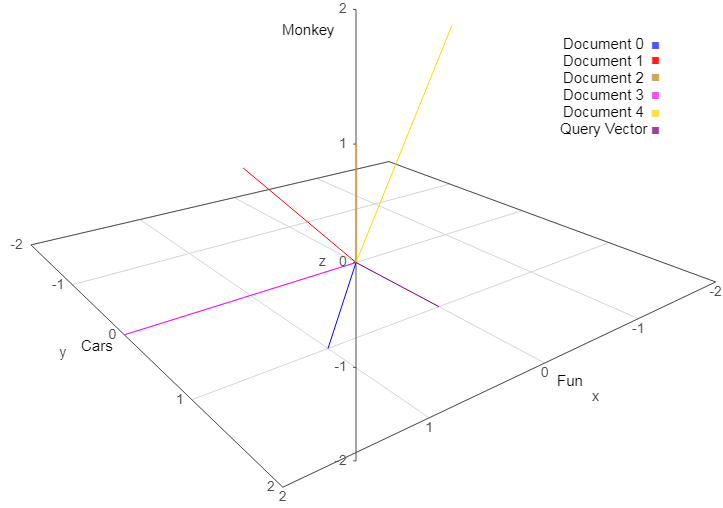
\includegraphics[width=5in]{imgs/withquery3d.png}
\caption{A Visual Representation of Table 1's Document Vectors}
\label{img:sansquery}
\end{figure}

Using  \autoref{table:MathToySet} as an example, The first dimension in the vector representation here corresponds to the term "cars", the second to "fun" and the third to "monkey". The normalized vectors' components are then scaled such that the vector has a length of one under the Euclidean norm. We do this to make future computation easier as it doesn't change the semantic meaning of the vector, since its the geometric relationship between the vectors rather than the vectors themselves that contains the information we need.

%TODO:CREATE MATRIX A FOR Example above for using in the rest of the pape 

Storing the information this way allow us to quickly and easily determine the semantic similarity between documents in a quantitative way. It also allows us to determine those documents which are closest in semantic meaning to a particular query, which is itself assigned a semantic meaning vector, thus creating a word-frequency-based search engine scalable to an arbitrarily large corpus of arbitrary term complexity.

% TODO: visual represnetation of Table 1, with highlighting for the meaning of each section


\subsection{Querying}\label{subsec:querying}

A query to the database is a string of terms. This string, just like the documents, can be represented as a vector of \(n\) dimensions. For example, using the vector space from \autoref{table:MathToySet}, a query for "fun" would have the vector representation
\begin{equation}
    q_1 = (0, 1, 0)^T. \notag
\end{equation}
A query vector will point in the direction of its semantic meaning, and the document vectors with the least distance to the normalized query vector will correspond to the most topically relevant documents in the corpus.

% TODO: Other visual representation

The geometry of the space can then be exploited to efficiently find which vectors are closest. The cosine of the angle between two unit vectors in the vector space corresponds to how close they are in the space. The closer the cosine is to 1, the closer they are. For a query vector \(q\) and any document vector \(a_j\), the cosine of the angle can be calculated using

\begin{equation}\label{eq:cosine}
    \cos{\theta_j} = \frac{a_j^T q}{\|a_j\|_2 \|q\|_2},
\end{equation}

where \(\|x\|_2\) is the Euclidean norm. Thus, to execute a query, simply calculate the cosine between the query's vector and each document's vector representation using \autoref{eq:cosine}, and the results with the highest cosine values will be the most relevant.


\subsection{Singular Value Decomposition}\label{subsec:SVD}
% Having thus explained the vector space model and how querying can be completed, 
We will now describe how to use 
Singular Value Decomposition (SVD) in the context of a vector space model IR. In this section, we will introduce SVD and its key 
concepts. In future sections, we will show how it is used for IR.

SVD is a factorization of a matrix that breaks up a matrix into three separate matrices such that $\matr{A} = \matr{U}\matr{\Sigma}\matr{V}^T$, 
where $\matr{U}$ and $\matr{V}$ are square matrices and $\matr{\Sigma}$ is a diagonal matrix. A pictorial representation of this can be seen in \autoref{fig:svdA}
\begin{figure}[H]
    \centering
    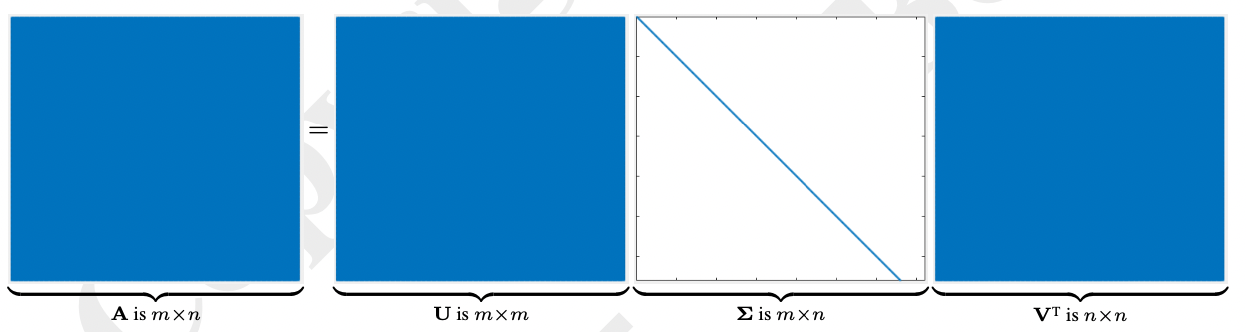
\includegraphics[width=\textwidth]{./imgs/SVD.jpg}
    \caption{SVD Representation of $\mtrA$ (image from \cite{svdImage})}
    \label{fig:svdA}
\end{figure}
 $\mtrSig$ contains the singular values, which are the square roots of the eigenvalues, of $\matr{A}^T\matr{A}$. 
 These singular values will be represented in this paper as $\sigma$, and they are ordered on the diagonal in increasing 
 order such that $\sigma_{11} \geq \sigma_{22} \geq \dots \geq \sigma_{\text{min}(m,n)}$. In addition, the columns of $\mtrV$ 
 represent eigenvectors of $\matr{A}^T\matr{A}$. Similarly, the columns of $\mtrU$ contain the eigenvectors of $\matr{A}\matr{A}^T$. 

  
 Physically interpreted, the columns of $\matr{V}$ represent a basis of $\RR^n$ and the columns of $\matr{U}$ represent a basis of $\RR^m$. This means that $\mtrU$ and $\mtrV^T$ are orthogonal matrices. Furthermore, $\mtrA$ represents a way to map basis $\mtrV$ to basis $\mtrU$, meaning:
 \begin{align*}
     \mtrA\mvec{x} &= \mtrA( c_1\mvec{V}_1 + c_2\mvec{V}_2 + \dots + c_n\mvec{V}_n)\\
     &= c_1\sigma_{11}\mvec{U}_1 +  c_2\sigma_{22}\mvec{U}_2 + \dots + c_n\sigma_{mm}\mvec{U}_m 
 \end{align*}


\subsection{Low-Rank Approximation}\label{subsec:lowRankAppx}
We must now discuss two practical points in using the vector space model: dealing with uncertainties as well as methods to
make querying computationally cheaper.

As one can imagine, there is no "perfect" way to create a matrix database. There will be variance in how the 
dictionary of terms is created, how term frequency is calculated, and more. Thus, we could theoretically define an uncertainty 
matrix $\mtrE$, which could correct for differences in opinion or incomplete information such that the database matrix 
is more accurately represented by $\mtrA'=\mtrA + \mtrE$. Extrapolating from this, we may then conclude that $\mtrA$ is only closely representative
of the "perfect" database matrix, and thus there would be a number of matrices that would represent the data just as well.

Let us assume that $\mtrA$ has rank $r_A$ and that $\mtrA'$ has rank $r_{A'}$ such 
that $r_{A'} < r_A$. Given the assumption that $\mtrA'$ is a better representation of the true data, this allows us to conclude the data has a matrix approximation of rank $r_{A'}$. Thus, it seems as though 
rank reduction of the matrix database may help remove noise from the representation. 
At the very least, it would allow for reasonably accurate querying using far less compute power.
To implement this in practice such that the matrix approximation does not lose too much data, we must now establish a few concepts. 
%TODO keep this in?

\subsubsection{Creating a Rank k Approximation with an SVD}
First, we need a way to create a low rank-$k$ approximation of $\mtrA$. To do so we will use the concept of SVD, and define a rank-approximation matrix $\mtrAK = \mtrUK\mtrSigK\mtrVK^T$. Here, $\mtrUK$ is a $m \times k$ matrix of the first $k$ columns  of $\mtrU$, $\mtrVK$ is a  $k \times n$ matrix of the first $k$ columns of $\mtrV$, and $\mtrSig$ is a $k \times k$ diagonal matrix of with the $k$ largest singular values of $\mtrA$. This is pictorially represented in \autoref{fig:isvdA}.
\begin{figure}[H]
    \centering
    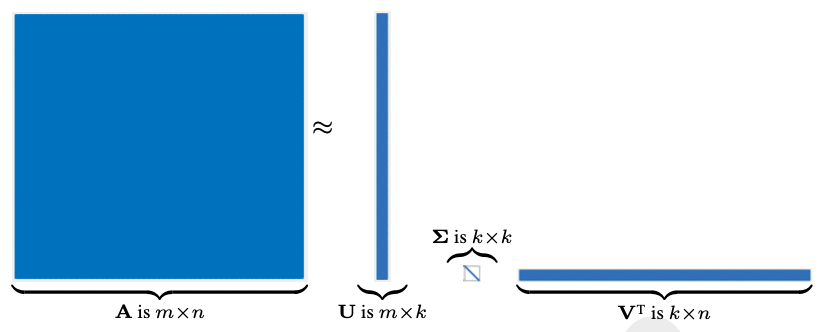
\includegraphics[width=0.6\textwidth]{./imgs/ISVD.jpg}
    \caption{Rank-$k$ Representation of $\mtrA$ (image from \cite{svdImage})}
    \label{fig:isvdA}
\end{figure}
 Note that, as stated before, through this approximation, we can represent $\mtrA$ using fewer values, which can conserve computational resources.
This works because the singular values (and in turn their corresponding eigenvectors) are in decreasing order, so we can assume that the large elements of $\mtrSig$ and the corresponding columns in $\mtrU$ and $\mtrV$ matter the most in representing $\mtrA$. Mathematically:
 \begin{align*}
     \mtrA\mvec{x} &= c_1\sigma_{11}\mvec{U}_1 +  c_2\sigma_{22}\mvec{U}_2 + \dots + c_n\sigma_{mm}\mvec{U}_m \\
     &\approx c_1\sigma_{11}\mvec{U}_1 +  c_2\sigma_{22}\mvec{U}_2 + \dots + c_n\sigma_{kk}\mvec{U}_k \tag{where $k < m$} 
 \end{align*}

 \subsubsection{A Method to Compare Matrices}
Next, to determine how much information is lost in the approximation, we must be able to compare the relative sizes of the matrices. To do this, we use the generalization of the Euclidean norm, the Frobenius matrix norm.

Just as we might divide the Euclidean norms of two vectors to determine the ratio of their lengths, we can do the same with the Frobenius norm. Thus, given some matrices $\matr{Y}$ and $\matr{X}$, $\|\matr{X}\|_F / \|\matr{Y}\|_F =$ the ratio of the size between the two. The smaller the ratio, the "smaller"
$\matr{X}$ is as compared to $\matr{Y}$.

 
 With this in mind, let us now derive a computationally efficient way to find the Frobenius norm of an SVD matrix.
 First, let us assume we have a real $t \times d$ matrix $\matr{Y}$ . We can define the Frobenius norm in terms of the matrix trace Trace($\matr{Y}$), which is the sum of the diagonals of the matrix $\matr{Y}^T\matr{Y}$, since
\begin{equation} \label{eq:forbTrace}
\begin{aligned}
     \|\matr{Y}\|_F = \sqrt{\sum_{i=1}^t \sum_{j=1}^d  y_{ij}y_{ij}} \\
                    = \sqrt{\text{Trace}(\matr{Y}^T\matr{Y})} \\
                    = \sqrt{\text{Trace}(\matr{Y}\matr{Y}^T)}
\end{aligned}
\end{equation}
Now we must prove that if the matrix multiplication is defined, multiplying any matrix by an orthogonal matrix does not change the Frobenius norm. Using our $\matr{Y}$ and a $t \times t$ orthogonal matrix $\matr{O}$, it follows from \autoref{eq:forbTrace} that:
\begin{equation} \label{eq:froboOrtho1}
\begin{aligned}
    \|\matr{O}\matr{Y}\|_F &= \sqrt{\text{Trace}((\matr{O}\matr{Y})^T(\matr{O}\matr{Y}))}   \\
            &= \sqrt{\text{Trace}(\matr{Y}^T\matr{O}^T\matr{O}\matr{Y})} \\ 
            &=  \sqrt{\text{Trace}(\matr{Y}^T\matr{Y})}  \\
            &=  \|\matr{Y}\|_F 
\end{aligned}
\end{equation}
It follows from a similar argument that given a $ d\times d$ orthogonal matrix $\matr{V}$:
\begin{equation} \label{eq:frobFull}
    \|\matr{Y}\matr{V}\|_F = \|\matr{Y}\|_F 
\end{equation}
Using these results, since $\mtrU$ and $\mtrV$ are orthogonal, it follows from \autoref{eq:froboOrtho1} and \autoref{eq:frobFull}, that the Frobenius norm of a SVD is:
\begin{equation} \label{eq:froboFinal}
\begin{aligned}
    \|\mtrA\|_F &= \|\mtrU\mtrSig\mtrV^T\|_F   \\
        &= \|\mtrSig\mtrV^T\|_F \\
        &= \|\mtrSig\|_F \\
        &= \sqrt{\sum_{i=1}^{r_A}\sigma_{ii}^2}
\end{aligned}
\end{equation}
Thus, once we compute the SVD of a matrix, we simply need to sum the squares of the singular values, which makes computing the Frobenius norm of our matrix much faster. 

\subsubsection{Determining a Valid Rank for Rank Approximation}\label{subsubsec:validrank}
Now that we have a mechanism to compare size, we need one final piece, which will then allow us to create a heuristic to choose which rank-$k$ approximation we ought to use to represent our data set. 

For this computation, we will need to be able to find $\|\mtrA-\mtrAK\|_F$  as this gives the "size"
of the information loss/change in using the rank-$k$ approximation, which we can then compare against the full matrix. This derivation is outside the scope of this project, and thus we will simply state that according
to the Eckart–Young–Minsky Theorem \cite{eckartYoung}:
\begin{equation}\label{eq:frobDiff}
    \|\mtrA-\mtrAK\|_F = \sqrt{\sum_{d=k+1}^{r_A}\sigma_{dd}^2}
\end{equation}
Hence, rather than take the difference and then compute the entire Frobenius norm, we need only use the singular values left over from the partition.

Now we can put this all together to determine a computationally efficient way 
to find an acceptable approximation of our database. We use the following algorithm:
\begin{enumerate}
    \item \textit{denominator} := $\|\mtrA\|_F$ using \autoref{eq:froboFinal} %Todo, add the rank thing
    \item For $x:=r_A$ until $x=1$:
    \begin{enumerate}
        \item \textit{numerator} := $\|\mtrA-\mtrAK\|_F$ using \autoref{eq:frobDiff}
        \item \textit{result} :=  $\frac{\textit{numerator}}{\textit{denominator}}$ 
        \item If \textit{result} is too large (in our case $\geq 0.4$), halt the algorithm and use $k=x-1$ as the rank for our approximation
        \item $x:=x-1$
    \end{enumerate}
\end{enumerate}

As seen above, we first store the Frobenious norm of the matrix, so we only have to compute it once.
Then, for each value of $k$, we compute the Frobenius norm of the difference between
our approximation and the actual matrix. Then we compute the ratio of the difference to the actual matrix, and this then tells us how small our change in the data size would be if we were to use the approximation in place of the true matrix. The larger the size, the more data we are potentially losing. Thus, when that change becomes too large (for some agreed bound), we know what approximation we can use. We can now define our querying method in terms of a rank-$k$ approximation of the
database matrix.

Note that the cutoff value is generally matrix/implementation specific and can be difficult to decide upon. For the purposes of this paper, we will assign the limit of 0.4 as we are willing to sacrifice some accuracy in pursuit of computational ease. Know however, that is is more usual to use a value of 0.2 or smaller \cite{berry99}.


\subsection{Using The SVD Rank k Approximation for Querying}
Finally, we can determine how to resolve a query using this approximation.
Let us define $e_j$ as the $j$th column of the $n \times n$ identity matrix, so that the $j$th column of
$\mtrAK$ is equivalent to $\mtrAK e_j$. Building upon the querying method described in \autoref{subsec:querying}, we thus could 
say that the cosine of the angle between a query $q$ and the $j$th approximated document vector is
\begin{equation}\label{eq:rankCos}
\begin{aligned}
    \cos\theta_j  &= \frac{(\mtrAK e_j)^Tq}{\|\mtrAK e_j\|_2 \|q\|_2 } \\
                &= \frac{(\mtrUK\mtrSigK\mtrVK^T e_j)^Tq}{\|\mtrUK\mtrSigK\mtrVK^T e_j\|_2 \|q\|_2 } \\
                &= \frac{e_j^T\mtrVK\mtrSigK (\mtrUK^Tq)}{\|\mtrUK\mtrSigK\mtrVK e_j\|_2 \|q\|_2 }        
\end{aligned}
\end{equation}

This is the equation with which we will compute our query results. 
%TODO add geometric explanantion of the colum space blah blah?





 